\documentclass[11pt]{jreport}
\setlength{\topmargin}{-15mm}
\setlength{\evensidemargin}{-2mm}
\setlength{\oddsidemargin}{3mm}
\setlength{\textheight}{24.5cm}
\setlength{\textwidth}{15cm}
%%
\usepackage[dvipdfm]{graphicx}
\usepackage{enumerate}

\usepackage{subfigure}

\usepackage{algorithm}
\usepackage{algorithmic}
\usepackage{bm} % $B?t<0$NCf$N(BBold (\bm{})
\usepackage{amsmath} % $B?t<0$NCf$N2~9T(B (\begin{gather} \\ )

\usepackage{listings,jlisting}

\renewcommand{\algorithmicrequire}{\textbf{Input:}}
\renewcommand{\algorithmicensure}{\textbf{Output:}}

\newcommand {\figref}[1] {$B?^(B\ref{#1}}
\newcommand{\tabref}[1] {$BI=(B\ref{#1}}
\newcommand{\argmax}{\operatornamewithlimits{argmax}}
\newcommand{\argmin}{\operatornamewithlimits{argmin}}

\renewcommand{\subfigtopskip}{1pt}
\renewcommand{\subfigbottomskip}{1pt}
\renewcommand{\subfigcapskip}{1pt}
\setlength{\floatsep}{6pt}           % $B?^I=$H?^I=$N4V$N%^!<%8%s(B
\setlength{\dblfloatsep}{6pt}        % $B",$NFsCJAH(B version
\setlength{\textfloatsep}{6pt}       % $B?^I=$HK\J8$N4V$N%^!<%8%s(B
\setlength{\abovecaptionskip}{-2pt}   % $B?^I=$N(B caption $B$H?^I=K\BN$N4V$N%^!<%8%s(B
\setlength{\belowcaptionskip}{2pt}   % $B?^I=$N(B caption $B2<It$N%^!<%8%s(B

\input amssym.def

\author{$BEl5~Bg3X!!>pJsM}9)3X7O8&5f2J!!0pMU8&5f<<(B}
\title{$B<j@h%+%a%i$rMQ$$$?APOS%m%\%C%H$K$h$k(B\\
$B%^%K%T%e%l!<%7%g%s%7%9%F%`(B\\
$BA`:n<j=g=q(B}
%\date{2010/4/10}

\begin{document}
\setlength{\baselineskip}{1.5zw}

\maketitle

\tableofcontents


\chapter{$B%7%9%F%`35MW(B}

$BK\%5!<%S%9$O!$9)>l$G$NItIJ@0M}$r%$%a!<%8$7$?$b$N$G$"$k!%(B
$B6qBNE*$K$O<j@h$N%+%a%i$rMQ$$$F:n6HBf>e$NItIJ$rG'<1$7(B,
$BN><j$GH"$K@0M}$7$FF~$l$k5!G=$r<B8=$7$^$9!%(B
$B<j$rF0$+$9$3$H$GJ#?t$NBP>]J*$rG'<1!$N><j$N43>D$r9MN8$7$F(B
$BF1;~$K%"%W%m!<%A$G$-$kBP>]J*$rA*Br$7$^$9!%(B

\begin{figure}[tbh]
 \begin{center}
  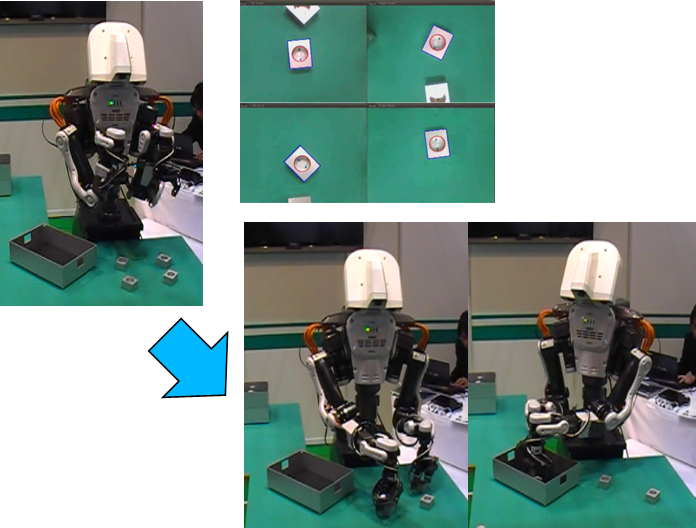
\includegraphics[width=1.0\linewidth]{figure/system.png}
  \caption{$B%5!<%S%9%$%a!<%8(B}
  \label{fig:system}
 \end{center}
\end{figure}

 \section{$BA4BN$N%b%8%e!<%k9=@.(B}

 $B0J2<$K!$K\%7%9%F%`$GMxMQ$9$k%b%8%e!<%k$N0lMw$r<($7$^$9!%(B
 $B$3$l$i$rF~<j$7!$<B9T2DG=$J4D6-$r@0$($F$/$@$5$$!%(B
\begin{itemize}
 \item app-recog
 \item CameraComp
 \item (LoadPictureComp)
 \item iv\_plan\_hironx
 \item HiroNXInterface
\end{itemize}
$B%U%!%$%k%7%9%F%`>e$N>l=j$OI,$:$7$b=EMW$G$O$J$$$G$9$,!$(B
$B#1$D$N%G%#%l%/%H%j$K$3$l$i$rCV$$$F$*$/$H!$K\%I%-%e%a%s%H$H$"$o$;$FM}2r$7(B
$B$d$9$$$G$9!%$3$l$i$N%b%8%e!<%k$O!$(B1$BBf$N7W;;5!>e$G<B9T$7$F$b!$F0:n@8@.It(B
$B$rJL$N7W;;5!$G<B9T$7$F$b$I$A$i$G$b9=$$$^$;$s!%(B
$BG'<1It$ODL?.Ii2Y$r9M$($k$H%+%a%i$,$D$J$,$C$F$$$k%[%9%H>e$G<B9T$9$k$3$H$r(B
$B?d>)$7$^$9!%(B

\begin{figure}[tbh]
 \begin{center}
  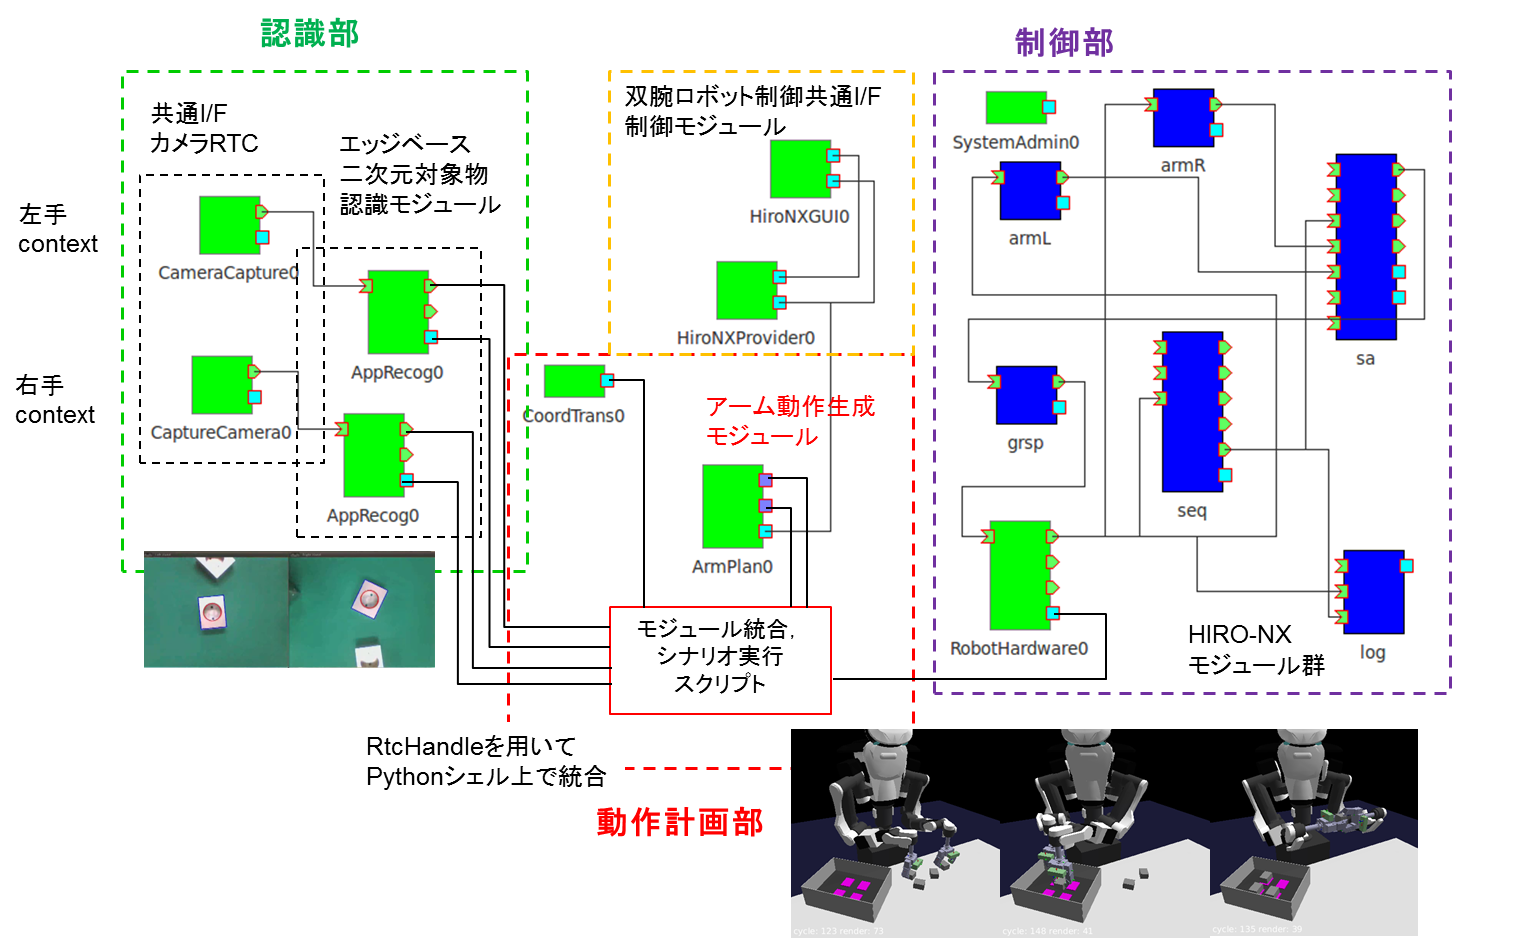
\includegraphics[width=1.0\linewidth]{figure/rtc_diagram.png}
  \caption{$BA4BN$N%b%8%e!<%k9=@.(B}
  \label{fig:rtc_diagram}
 \end{center}
\end{figure}


\section{$BG'<1It(B}

\subsection{$B%(%C%8%Y!<%9Fs<!85BP>]J*G'<1%b%8%e!<%k(B(AppRecog)}

http://openrtm.org/openrtm/ja/project/NEDO\_Intelligent\_PRJ\_HiroAccPrj\_5002

HiroNX$B$N<j@h$K<h$jIU$1$i$l$?(BUSB$B%+%a%i$GBP>]J*$rG'<1$9$k$?$a$KMxMQ$7$^$9!%(B
$BN><j@h$N%+%a%i$=$l$>$l$G%+%a%i%b%8%e!<%k$H$H$b$K<B9T$7$^$9!%(B
$B;H$$J}$O%b%8%e!<%kIUB0$N%I%-%e%a%s%H$r;2>H$7$F$/$@$5$$!%(B

\subsection{$B%+%a%i6&DL(BI/F$B=`5r$N2hA|%-%c%W%A%c%b%8%e!<%k(B(CameraComp)}

http://www-arailab.sys.es.osaka-u.ac.jp/CameraIF/

$BBg:eBg3X$K$h$j3+H/$5$l2hA|%-%c%W%A%c%b%8%e!<%k(BCameraComp$B$r%@%&%s%m!<%I!$(B
$B%3%s%Q%$%k$7$^$9!%MxMQJ}K!$O!$K\%b%8%e!<%k$N%I%-%e%a%s%H$*$h$S!$(B
$B>e5-(BAppRecog$BIUB0$N%I%-%e%a%s%H$r;2>H$7$F$/$@$5$$!%(B

\section{$BF0:n@8@.It(B}

\subsection{(VPython$BHG(B)HiroNX$BF0:n@8@.%b%8%e!<%k(B}

$BG'<17k2L$r@$3&:BI8$X$NJQ49!$(BHiroNX$B$NF0:n$N@8@.!$%?%9%/5-=R$r9T$J$&$?$a$K(B
$BMxMQ$7$^$9!%>\$7$/$O!$%b%8%e!<%kIUB0$N%I%-%e%a%s%H$r;2>H$7$F$/$@$5$$!%(B

\subsection{HiroNXInterface}

http://www.openrtm.org/openrtm/en/node/4645

$BAPOS%m%\%C%H$N@)8f%3%^%s%I$N6&DL%$%s%?%U%'!<%9$K=`5r$9$k(B
HiroNX$BMQ@)8f%b%8%e!<%k$G$9!%(B
$B>\:Y$K$D$$$F$O!$3+H/85$G$"$k;:6H5;=QAm9g8&5f=j$N%I%-%e%a%s%H$r;2>H$7$F$/(B
$B$@$5$$!%(B


\chapter{$B=`Hw(B}

$BI,MW$K1~$8$F%G%b4D6-!$%m%\%C%H$4$H$K0J2<$N:n6H$r9T$$$^$9!%(B

\section{$BNO%;%s%5$NM-L5!$%F!<%V%k$N9b$5(B}

$B<j<s$KNO%;%s%5$,$"$k>l9g$H$J$$>l9g$G!$%m!<%I$9$k%b%G%k$rJQ99$9$kI,(B
$BMW$,$"$j$^$9!%%5%s%W%k%W%m%0%i%`$O!$NO%;%s%5$,$"$k>l9g$K<j<s$N%j%s%/D9$rJQ99!$1_E{7A>u(B
$B$rA^F~$7$?$b$N$G$9!%NO%;%s%5$,$J$$>l9g$O!$(B
\verb|HiroNX|$B%$%s%9%?%s%9$r@8@.$9$k$H$-$K!$%*%W%7%g%s(B\verb|forcesensors=False|$B$r;XDj$7$^$9!%(B

$B$^$?!$%7%_%e%l!<%?Fb%7!<%s$O(Biv\_plan/src/scene\_objects.py$B$GDj5A$5$l$?(B
Python$B$N%G!<%?9=B$$r2r<a$7$F@8@.$5$l$^$9!%(B
$B%G%U%)%k%H$G9b$5(B700[mm]$B$NElBg;EMM%F!<%V%k(B(table\_scene())$B$H(B
$B9b$5(B735[mm]$B$N(BAIST$B;EMM%F!<%V%k(B(table\_scene\_aist())$B$,MQ0U$5$l$F$$$^$9!%(B
$B$=$l0J30$N%7!<%s$r:n@.$7$?$$>l9g$O!$(Bscene\_objects.py$B$r;29M$K!$%7!<%s5-=R(B
$B$r:n@.$7!$(Benv.load\_scene()$B$G4D6-$K%m!<%I$7$F$/$@$5$$!%(B

\section{$B%-%c%j%V%l!<%7%g%s(B}

$B%m%\%C%H$N8DBN:9$r=$@5$9$k:n6H$G$9!%%+%a%i$NFbIt%Q%i%a!<%?$*$h$S!$%m%\%C(B
$B%H$N%j%s%/$KBP$9$k%+%a%i$N<h$jIU$10LCV$r7W;;$7$^$9!%(B
$B%G%U%)%k%HCM$O(BHiroNX14$B9f5!$N$b$N$G$"$j!$@:EY$r=P$9$K$O3F5!BN$4$H$K9T$&I,MW$,$"$j$^$9!%(B

\subsection{$B%+%a%i$N%-%c%j%V%l!<%7%g%s(B}

RT-middleware$B$N%3%s%]!<%M%s%H$G$b(BROS$B$N%N!<%I$G$b$h$$$N$GC14c%+%a%i$N%-%c(B
$B%j%V%l!<%7%g%s$r9T$$!$(BCameraComp$B$,FI$_9~$a$k$h$&$K$7$^$9!%K\%7%9%F%`$K$*(B
$B$$$F!$(Brun.sh$B%9%/%j%W%H$G(BRTC$B$r5/F0$9$k>l9g!$(Bscripts$B%G%#%l%/%H%j$K$"$k(B
camera\_left.yml$B$*$h$S(Bcamera\_right.yml$B$K$=$l$>$l$N%+%a%i$NFbIt%Q%i%a!<(B
$B%?$r5-=R$7$^$9!%(B
$B$=$N8e!$%(%C%8%Y!<%9Fs<!85BP>]J*G'<1%b%8%e!<%k$K$*$$$F!$BP>]J*$N0LCV!$5w(B
$BN%$,@5$7$/=PNO$5$l$F$$$k$+$I$&$+3NG'$7$F$*$$$F$/$@$5$$!%(B
$B%-%c%j%V%l!<%7%g%s$r9T$J$&$H$-$O!$0J2<$N4X?t$r<B9T$7$F<j@h%+%a%i$r@5LL$K(B
$B8~$1$k(B(\figref{fig:camcalib_pose})$B$H:n6H$,MF0W$K$J$j$^$9!%(B

\begin{lstlisting}
 $ ipython
 >>> from hironx_calib import *
 >>> handcam_calib_pose()
 >>> sync()
\end{lstlisting}

\begin{figure}[tbh]
 \begin{center}
  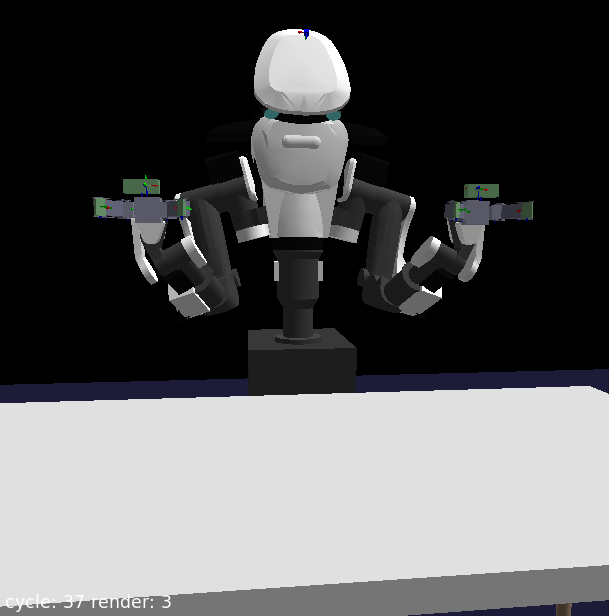
\includegraphics[width=0.5\linewidth]{figure/camcalib_pose.png}
  \caption{$B%+%a%i%-%c%j%V%l!<%7%g%sMQ$N;Q@*(B}
  \label{fig:camcalib_pose}
 \end{center}
\end{figure}

\subsection{$B%+%a%i<h$jIU$10LCV$N%-%c%j%V%l!<%7%g%s(B}

$B<!$K!$%+%a%i$N<h$jIU$10LCV$r7W;;$7$^$9!%(B
$B%-%c%j%V%l!<%7%g%s%W%m%0%i%`$O!$3X=,%G!<%?$H$7$F%m%\%C%H$N3F;Q@*$K$*$1$k(B
$B%A%'%C%+!<%\!<%I$N;Q@*$rF~NO$H$7$^$9(B(\figref{fig:handeye_calib})$B!%%A%'%C(B
$B%+!<%\!<%I$NG'<1$K$O(BROS$B$N(Bcheckerboard\_detection$B%N!<%I$r;HMQ$7!$(Btf$B$H$7$F(B
publish$B$5$l$?%A%'%C%+!<%\!<%I$N;Q@*$r(Bpython$B%W%m%0%i%`$G<u?.$7$^$9!%6qBN(B
$BE*$J<j=g$O!$IUO?$K5-:\$7$^$9!%(B
\begin{figure}[tbh]
 \begin{center}
  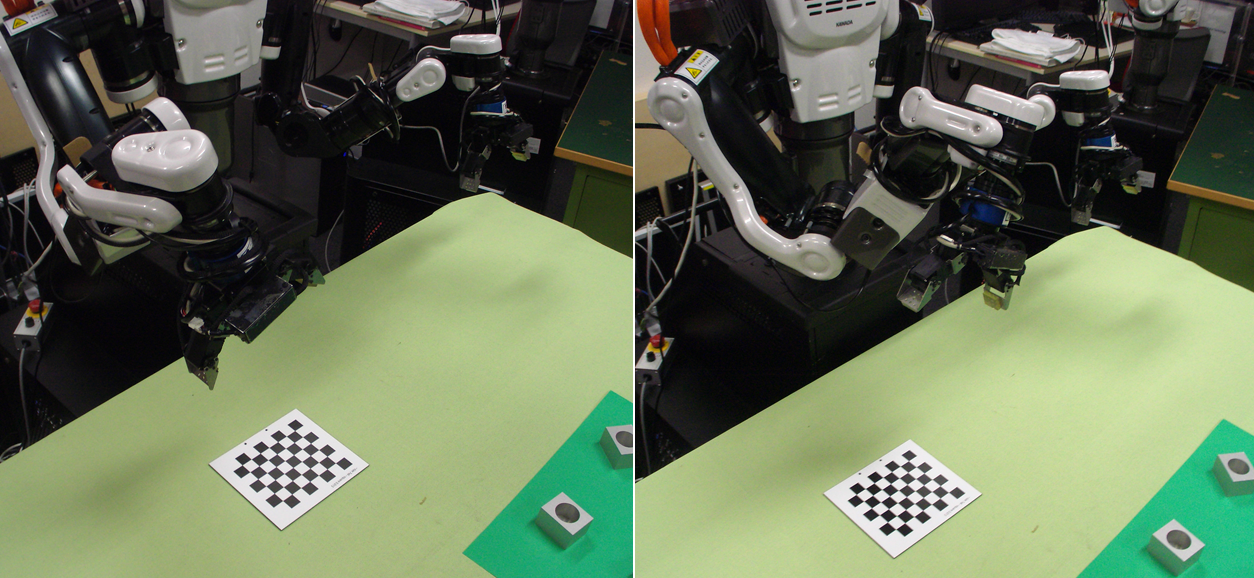
\includegraphics[width=0.8\linewidth]{figure/handeye_calib.png}
  \caption{$B<j@h$rF0$+$7$?%A%'%C%+!<%\!<%I$N8!=P(B}
  \label{fig:handeye_calib}
 \end{center}
\end{figure}

\chapter{$B%G%b$N<B9T(B}

\section{$B@)8f7O%b%8%e!<%k$N5/F0$H@\B3(B}

\begin{lstlisting}
 $ cd iv_plan/scripts
 $ ./run-hironx-interface.sh
\end{lstlisting}
$B$3$l$K$h$j!$N><j$KBP1~$9$k%+%a%i!$G'<1%b%8%e!<%k!$(BHiroNXInterface$B@)8f%b(B
$B%8%e!<%k$,5/F0!$@\B3$5$l!$$5$i$K3F%b%8%e!<%k$,(Bactivate$B$5$l$^$9!%(B
HiroNXInterface$B%b%8%e!<%k$O5/F08e(BGUI$B>e$N!V(BRTC Status$B!W$,NP$K$J$C$?>uBV$G(B
$B!V(BSet up Robot$B!W%\%?%s$r2!$7!$(BRTC$B$^$o$j$N=i4|2=$r9T$&I,MW$,$"$kE@$KCm0U$7(B
$B$F$/$@$5$$!%5/F0$7$?(BGUI$B$+$i0J2<$r<B9T$7$F$*$-$^$9!%(B
\begin{enumerate}
 \item $B%8%g%$%s%H%-%c%j%V%l!<%7%g%s(B
 \item $B=i4|;Q@*$X0\9T(B
 \item $B;X$N%5!<%\%*%s!!(B($B$D$$$G$K3+JDF0:n3NG'(B)
\end{enumerate}

\section{$BG'<17O%b%8%e!<%k$N5/F0$H@\B3(B}

$B<!$K!$(BHiroNX$BN><j$N<j@h%+%a%i$N%-%c%W%A%c5Z$S!$(BAppRecog$BG'<1%b%8%e!<%k$r5/(B
$BF0$7$^$9!%:81&$GF1$8L>A0$N%3%s%]!<%M%s%H72$r5/F0$9$k$?$a!$JL!9$N(BRTC$BL>A0(B
$B6u4V$K5/F0$7$^$9!%(B
\begin{lstlisting}
 $ ./run.sh
\end{lstlisting}
$B$3$3$G!$:81&$N%+%a%i$,5U$K$J$C$F$$$J$$$+$I$&$+3NG'$7$F$/$@$5$$!%(B
$B5U$K$J$C$F$$$k>l9g$O!$(BCaptureCameraLeft.conf$B$H(B
CaptureCameraRight.conf$B$K5-=R$7$F$"$k(Bconf.default.int\_camera\_id$B$NHV9f$r(B
$B5U$K$7$F!$(Brun.sh$B$r:F<B9T$7$F$/$@$5$$!%(B
$B:81&$=$l$>$l$N%b%8%e!<%k72$O5/F0$7$?C<Kv$G(BCtrl+c$B$r2!$9$3$H$G=*N;$7$^$9!%(B

iv\_plan/scripts$B$K$"$k%9%/%j%W%H$O!$%m!<%+%k$N%U%!%$%k%7%9%F%`Hs0MB8$JJ}(B
$BK!$G%b%8%e!<%k$N>l=j$r8!=P$9$k$?$a!$(BROS$B$N%3%^%s%I$G$"$k(Brospack$B$r;H$$$^$9!%(B
rospack$B$rMxMQ$G$-$J$$>l9g$O!$E,59!$%9%/%j%W%H$rJT=8$9$k$+F1Ey$N5!G=$r<B(B
$B8=$9$k%3%^%s%I$KCV$-49$($F$/$@$5$$!%(B
$B$b$7!$%3%s%]!<%M%s%H$,>e<j$/@\B3$*$h$S(Bactivate$B$5$l$J$$>l9g$O!$(B
./comcon.sh$B$*$h$S(B./comact.sh$B$r:FEY<B9T$7$F$_$F$/$@$5$$!%(B

$B%+%a%i$,G'<1$G$-$F$$$J$$2DG=@-$,$"$k>l9g$K$O!$(Bxawtv$B%3%^%s%I$J$I$G%+%a%i<+(B
$BBN$,G'<1$5$l$F$$$k$+3NG'$7$F$/$@$5$$!%(B
$BG'<14X78$N%b%8%e!<%k$rEPO?$9$k%M!<%`%5!<%P$O(Bscripts$B%G%#%l%/%H%j$N(B
rtc\_left.conf$B$*$h$S(Brtc\_right.conf$B$G;XDj$7$^$9!%(B

\section{$BF0:n@8@.7O%b%8%e!<%k$N5/F0$H%b%8%e!<%k4VDL?.$N3NG'(B}

$B0J2<$N%3%^%s%I$G%G%b%W%m%0%i%`$r5/F0$7!$(B
\begin{itemize}
 \item HiroNX$BK\BN$N%b%8%e!<%k$HDL?.$7!$4X@a3QEY$N<hF@$*$h$S!$F0:n%3%^%s%I(B
       $B$NAw?.$r9T$J$&$3$H$,$G$-$k$3$H(B
 \item $BG'<14o$HDL?.$7G'<17k2L$r<hF@$G$-$k$3$H(B
\end{itemize}
$B$r3NG'$7$^$9(B.
\begin{lstlisting}[label=src:branch]
 $ cd iv_scenario/src
 $ ipython demo_wexpo.py

 >>> rr.get_joint_angles() # $B<B5!$N4X@a3QEY$r<hF@(B
 >>> r.prepare()           # $B%7%_%e%l!<%?$N%b%G%k$N;Q@*$rJQ99(B
 >>> sync()                # $B<B5!$r%b%G%k$K$"$o$;$k(B($B<B5!$,F0$/$N$GCm0U(B)

 $B?^(B???$B$N$h$&$K!$G'<1$G$-$k0LCV$KBP>]J*$rCV$$$F(B
 >>> rr.detect(sensor='rhandcam') # $B1&<j%O%s%I%+%a%i$G$NG'<1(B
 >>> rr.detect(sensor='lhandcam') # $B:8<j%O%s%I%+%a%i$G$NG'<1(B

 $BG'<1$7$?8e!$$=$N7k2L$r@$3&:BI8$X$NJQ49$9$k(B
 >>> detect(sensor='rhandcam')
 >>> detect(sensor='lhandcam')

 >>> f = detect(sensor='rhandcam')
 >>> show_frame(f) # $BG'<17k2L$NI=<((B
 # $B%7%_%e%l!<%?Fb$GG'<10LCV$KH"(BA0$B$r0\F0$5$;$k(B
 >>> env.get_object('A0').locate(f) 
\end{lstlisting}
$B%b%8%e!<%k$HDL?.$G$-$J$$>l9g$O!$(Biv\_scenario/src$B$K$"$k(B
rtc.conf$B$G@5$7$/%M!<%`%5!<%P$,;XDj$5$l$F$$$k$+!$$^(B
$B$?!$(Biv\_scenario/interface\_wexpo.py$B$K=q$+$l$F$$$k3F%b%8%e!<%k$N%Q%9$,@5(B
$B$7$$$+$I$&$+3NG'$7$F$/$@$5$$!%(B

\section{$B%G%b$N<B9T(B}

\figref{fig:four_parts_on_the_table}$B$N$h$&$K:n6HBf$KBP>]J*$r(B4$B$DJB$Y!$(B
 $B:n6HBf>e$GN><j$rF0$+$7!$BP>]J*$r8!=P$G$-$k$+$I$&$+$r3NG'$7$F$_$^$9!%(B

\begin{lstlisting}
 >>> look_for()
\end{lstlisting}
 $B>e<j$/8!=P$G$-$l$P!$%7%_%e%l!<%?Fb$NH"(B4$B$D$,@5$7$$0LCV$K0\F0$7$^$9(B
 (\figref{fig:look_for}(a))$B!%(B
 (b)$B$G$O(B1$B$D!$(B(c)$B$G$O(B2$B$DG'<1$K<:GT$7$F$$$^$9!%(B
 $B>e<j$/8!=P$5$l$J$$$H$-$O!$2hA|Cf$GBP>]J*$,@5$7$/G'<1$5$l$F$$$k$+%A%'%C(B
 $B%/$7$F$/$@$5$$!%(B

 $B8!=P;~$N=i4|0LCV$X%m%\%C%H$N;Q@*$r;}$C$F$$$-$?$$$H$-$K$O(B,
$B0J2<$N%3%^%s%I$r<B9T$7$^$9!%(B
\begin{lstlisting}
 >>> go_scan_pose()
\end{lstlisting}

\begin{figure}[tbh]
 \begin{center}
  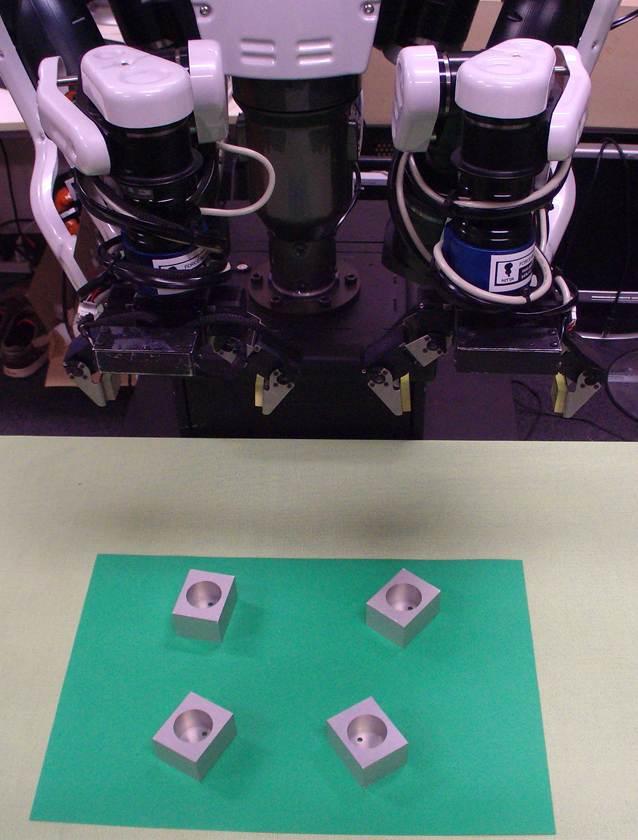
\includegraphics[width=0.45\linewidth]{figure/four_parts_on_the_table.jpg}
  \caption{$B#4$D$NItIJ$rJB$Y$?>uBV(B}
  \label{fig:four_parts_on_the_table}
 \end{center}
\end{figure}
\begin{figure}[tbh]
 \begin{center}
  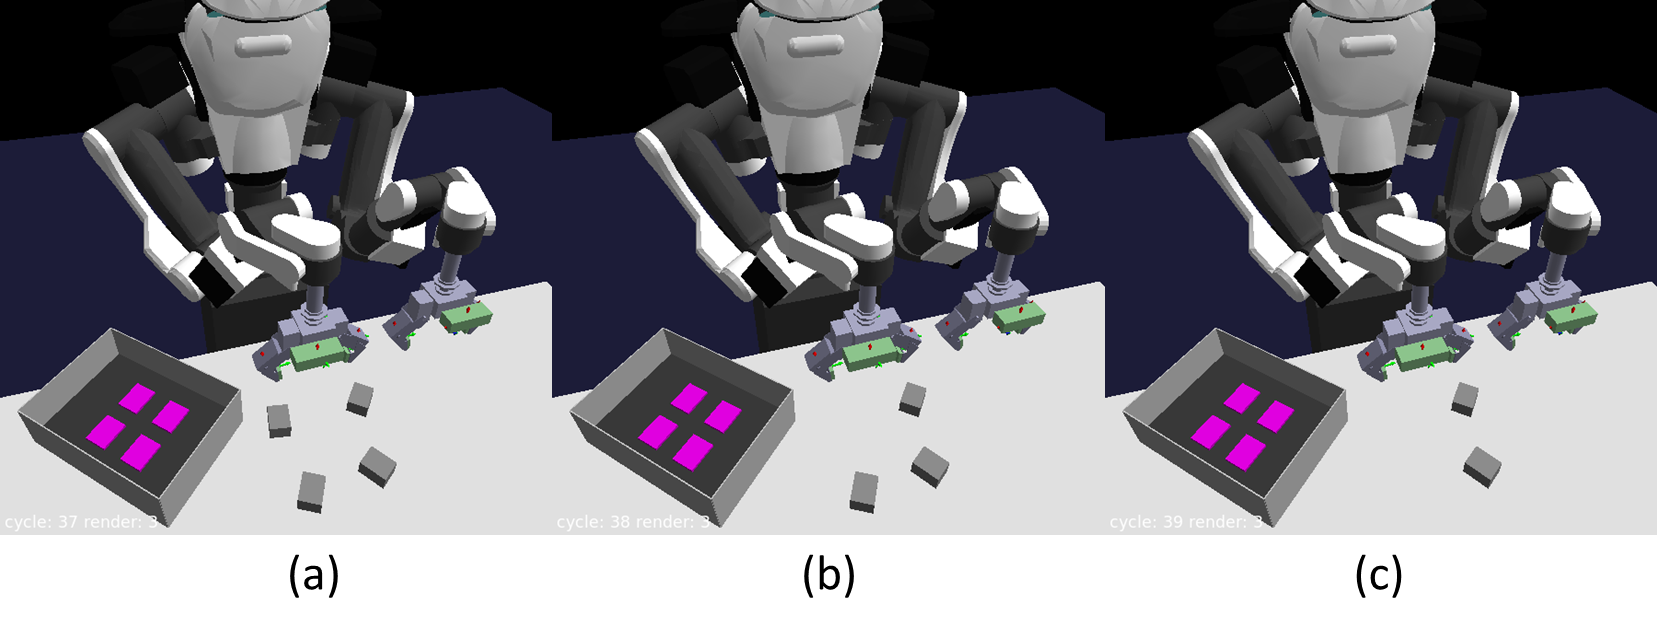
\includegraphics[width=1.0\linewidth]{figure/look_for.png}
  \caption{$B:n6HBf>e$NBP>]J*G'<17k2L(B}
  \label{fig:look_for}
 \end{center}
\end{figure}

 $B$3$l$G=`Hw$,@0$C$?$N$G!$<B:]$K%G%b$r<B9T$7$^$9!%(B
 \begin{lstlisting}
  >>> demo()
 \end{lstlisting}
 $B:n6HBf$r%9%-%c%s$7!$BP>]J*$r(B4$B$D8!=P$7$?8e!$(B
 $B:G=i$ON><j$G!$;D$j$N#2$D$OE,59;}$ABX$($r9T$J$C$FH"$KG[CV$7$^$9!%(B
 $BBP>]J*$r(B4$B$D8!=P$G$-$J$+$C$?$H$-$O!$F0:n$K$OF~$j$^$;$s!%(B

 % $B30It%b%8%e!<%k$H$NDL?.(B
 % >>> rr = MyHiroNxSystem(portdefs) # $B30It%b%8%e!<%k$H$NDL?.%$%s%?%U%'!<(B
 % $B%9%*%V%8%'%/%H$r:n@.(B


\newpage

\appendix
\chapter{$B%-%c%j%V%l!<%7%g%s%a%b(B}

checkerboard\_detection$B$*$h$S!$(Bcamera\_calibration$B%Q%C%1!<%8$rMQ0U$7$F$/(B
$B$@$5$$!%(BROS$B%N!<%I5/F0MQ$N(Blaunch$B%U%!%$%k%;%C%H$N%Q%C%1!<%8(BSense.tgz$B$r;H$$$^$9!%(B

\section{$B%+%a%i%-%c%j%V%l!<%7%g%s$N<j=g(B}

\begin{verbatim}
$ roslaunch Sense rhand.launch
$ rosrun camera_calibration cameracalibrator.py --size 7x10 --square
		0.025 image:=/rhand/usb_cam/image_raw
Sense/launch/rhand.launch$B$NFbIt%Q%i%a!<%?$r99?7$9$k(B
$ roslaunch Sense lhand.launch
$ rosrun camera_calibration cameracalibrator.py --size 7x10 --square
		0.025 image:=/lhand/usb_cam/image_raw
Sense/launch/lhand.launch$B$NFbIt%Q%i%a!<%?$r99?7$9$k(B
\end{verbatim}

\section{$B%+%a%i<h$jIU$10LCV%-%c%j%V%l!<%7%g%s$N<j=g(B}

\begin{enumerate}
 \item ROS$B$N%+%a%i%N!<%I$K$h$j2hA|$*$h$S>e5-%+%a%i%Q%i%a!<%?$,%H%T%C%/$H(B
       $B$7$F(Bpublish$B$5$l!$(Bcheckerboard detection$B%N!<%I$G$=$l$i$r(Bsubscribe
       $B$7!$?dDj$7$?(Btf$B$,(Bpublish$B$5$l$k$h$&$K$7$^$9!%(B \\
       \verb|$ roslaunch Sense rhand\_checkerboard.launch|
 \item $B4y$N>e$K%A%'%C%+!<%\!<%I$rCV$-$^$9(B
 \item $B<j$rF0$+$7$F3X=,%G!<%?$r<h$j$^$9!%(B
       \verb|$ cd iv_scenario/src|\\
       \verb|$ ipython|\\
       \verb|>>> from hironx_calib import *|\\
       \verb|>>> rr.connect()|\\
       \verb|>>> res = record_data(sensor='rhandcam')|\\
       $B$9$Y$F$N;Q@*$G!$%A%'%C%+!<%\!<%I$,;kLn$K<}$^$j!$(B
       $B0BDj$7$FG'<1$G$-$F$$$k$3$H$r3NG'$7$^$9(B(\figref{fig:handcalib_checkerboard})$B!%(B
 \item $B<j<s%j%s%/$+$i%+%a%i$X$N:BI8JQ49$r7W;;$7$^$9!%(B \\
       \verb|>>> f = calibrate(res, link='RARM_JOINT5_Link', tf0=r.Trh_cam)|
 \item $B7k2L$r3NG'$7$^$9!%(B \\
       \verb|>>> play_data(res, link='RARM_JOINT5_Link', tf=f)|
 \item $BLdBj$J$1$l$P(Bhironx\_params.py$B$N(BTrh\_cam$B$r99?7$7$^$9!%(B
 \item $B:8<j%+%a%i$K$D$$$F$bF1MM$K9T$$$^$9!%(B
\end{enumerate}

\begin{figure}[tbh]
 \begin{center}
  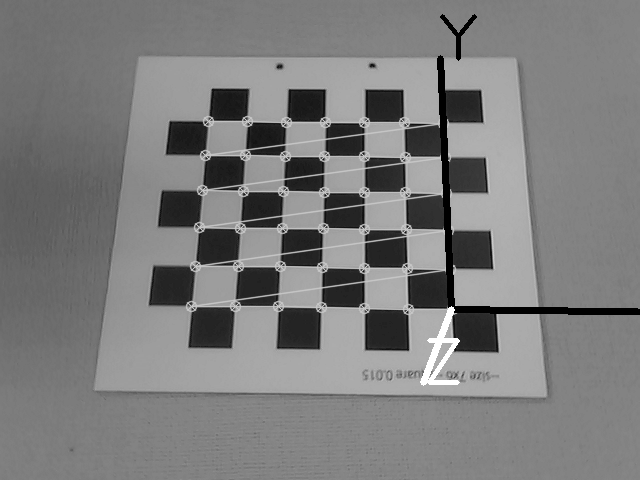
\includegraphics[width=0.6\linewidth]{figure/handcalib_checkerboard.png}
  \caption{checkerboard detector}
  \label{fig:handcalib_checkerboard}
 \end{center}
\end{figure}


% \addcontentsline{toc}{chapter}{$B;29MJ88%(B}
% \markboth{$B;29MJ88%(B}{$B;29MJ88%(B}
% \bibliographystyle{junsrt}
% \bibliography{p2009}

\end{document}
